\subsection{Image experiments}
For the image experiments we collected our dataset by downloading the complete galleries from around 30 artists.
Those artists were selected from the daily deviations of a random day and includes both premium and non premium members.
In total we downloaded around 5000 images. 
For each image we also stored the category information.
The dataset is unbalanced since some artists only have around 50 images, while other artists have over 500 images.
The top five categories are listed in table \ref{datasetstats} and the artists are listed in table \ref{userstats}(SHOULD IT HAVE ARTISTNAMES?).

\begin{table}
    \centering
    \begin{tabular}
        { | l | c | } 
        \hline
        Category & count \\
        \hline
        photography & 2244 \\ 
        customization & 906 \\ 
        traditional & 842 \\ 
        digitalart & 587 \\ 
        fanart & 239 \\ 
        \hline 
    \end{tabular}
    \caption{Dataset category statistics}
    \label{datasetstats}
\end{table}

\begin{table}
    \centering
    \begin{tabular}
        { | l | c | } 
        \hline
        Artist & count \\
        \hline
        Kitsunebaka91 & 293 \\ 
        gsphoto & 606 \\ 
        Knuxtiger & 56 \\ 
        RedPriestUsada & 88 \\ 
        etc. & 0 \\
        \hline
    \end{tabular}
    \caption{Dataset artist statistics}
    \label{userstats}
\end{table}

\subsubsection{Experiment 1: 1 vs all artists}
The first experiment using this toolkit is to find out if there are any artists in our dataset that uses an unique style.
Therefore this experiment is focused on using one artist as the positive class while all the other artists are in the negative class resulting in a two class problem.

For this experiment, three classifiers were used: kNN, Naive Bayes and the Nearest Mean classifiers.
The Nearest Mean classifier does not use any parameters but the other two classifiers do.
kNN uses 1 K 9 and Naive Bayes uses 6 Bins 24.
All the classifiers were trained on a training set which consists of 70 percent of the entire dataset and the F-measure is used to score the classifiers on how well they perform on each fold.
The average of the F-measure is used to assign the overall performance of a classifier and its parameter.
(SHOULD IT INCLUDE WHY NO SVM BECAUSE OF NOT IMPLEMENTED YET??)

\subsubsection{Experiment 1: Results}
The results from this experiment can be found in table \ref{ex1results}(SHOUDL IT INCLUDE ARTISTNAMES??). This table shows the top 10 classifiers with the average F-measure score using cross-validation on the train set. The table shows that the artists Kitsunebaka91 and gsphoto are multiple times in the top 10. 

\begin{table}
    \centering
    \begin{tabular}
        { | l | l | c | c } 
        \hline
        Artist & Classifier & Parameter & F-Measure \\
        \hline
        Kitsunebaka91 & Nearest Mean & - & 0.836  \\ 
        my-shots & kNN & 1 & 0.768 \\ 
        gsphoto & kNN & 7 & 0.752 \\ 
        gsphoto & Naive Bayes & 5 & 0.702 \\ 
        etc. & etc. & 0 & 0 \\
        \hline 
    \end{tabular}
    \caption{Dataset artist statistics}
    \label{ex1results}
\end{table}

%result: ranking of artists (some good, some bad), why the 2nd experiment is needed.
%Make sure that it is a initial experiment is made clear.
%This experiment should lead up to the 1 vs 1 artists experiment.

\subsubsection{1 vs 1 artists - classification performance}
The real experiment must give a message that this toolkit and deviantart is an interesting research area.

\subsection{Network experiments}
dataset

small world, describe network, identify core

\begin{figure}[htb]
  \centering
  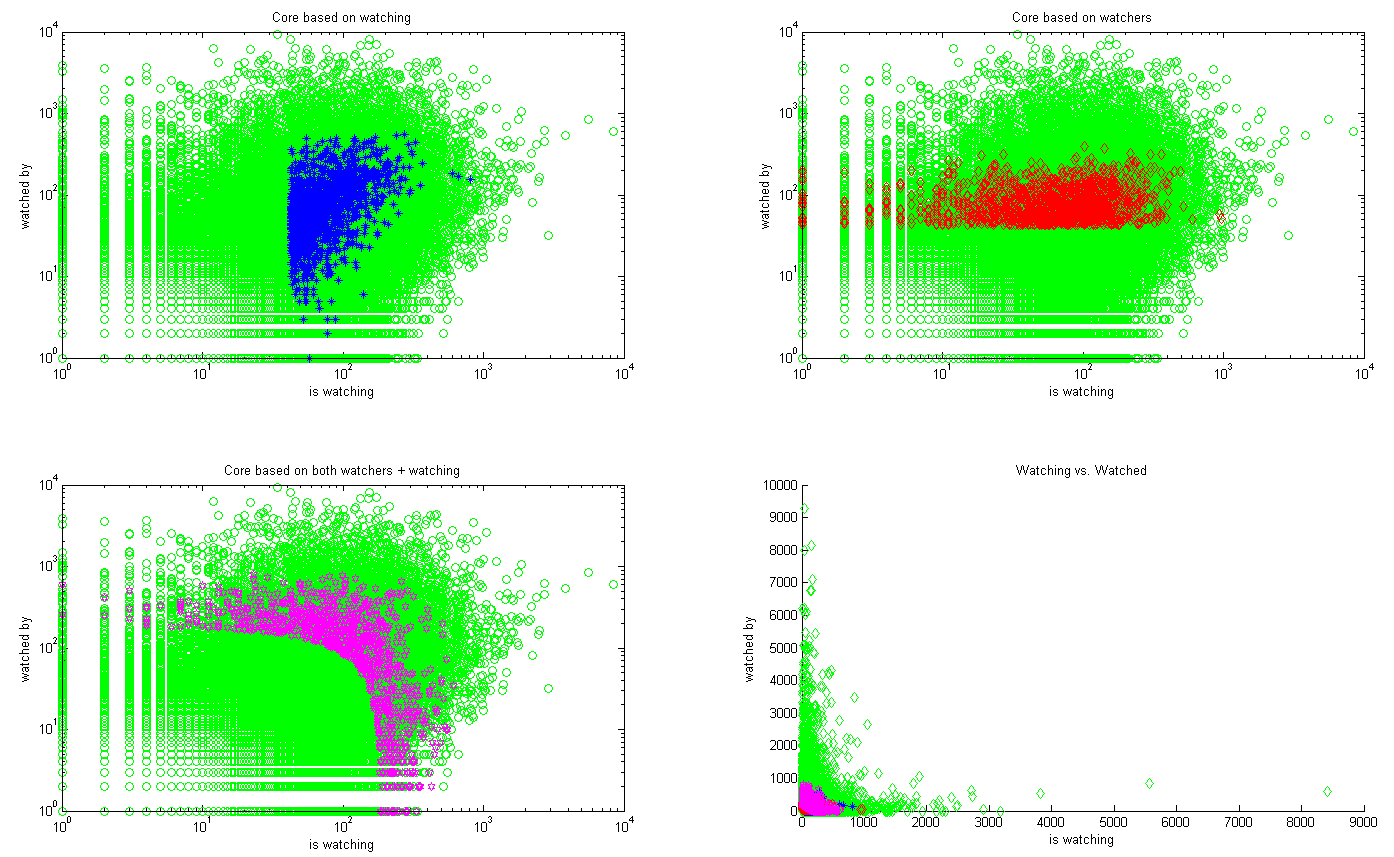
\includegraphics[width=1\linewidth]{img/core.png}
  \caption{Core network}
  \label{fig:results_core}
\end{figure}